\documentclass{article}
\usepackage{graphicx}
\usepackage{amsmath}
\usepackage[parfill]{parskip}
\usepackage{hyperref}
\usepackage[useregional]{datetime2}

\usepackage{biblatex}
\addbibresource{references.bib}

\usepackage[T1]{fontenc}
\usepackage{tgbonum}

\usepackage{listings}
\usepackage{xcolor}

% Define a custom color
\definecolor{backcolour}{rgb}{0.95,0.95,0.92}
\definecolor{codegreen}{rgb}{0,0.6,0}

% Define a custom style
\lstdefinestyle{myStyle}{
    backgroundcolor=\color{backcolour},   
    commentstyle=\color{codegreen},
    basicstyle=\ttfamily\footnotesize,
    breakatwhitespace=false,         
    breaklines=true,                 
    keepspaces=true,                 
    numbers=left,       
    numbersep=5pt,                  
    showspaces=false,                
    showstringspaces=false,
    showtabs=false,                  
    tabsize=2,
}

% Use \lstset to make myStyle the global default
\lstset{style=myStyle}

\graphicspath{ {./figures/} }

\title{COMP.SEC.110 Cyber Security II\\
    \large Practical Exercise: Secret-Encryption
}
\author{Cuong Nguyen\\ \href{mailto:cuong.nguyen@tuni.fi}{cuong.nguyen@tuni.fi} 
        \and Mahibul Momin\\ \href{mailto:mahibul.momin@tuni.fi}{mahibul.momin@tuni.fi}
}

\begin{document}
    
\maketitle
\tableofcontents
\newpage

\listoffigures
\newpage

% Content of report would be written here
% \section{Lab Tasks: Attacks}
\subsection{Task 1 --- Observing HTTP Request}
%
\begin{figure}
    \centering
    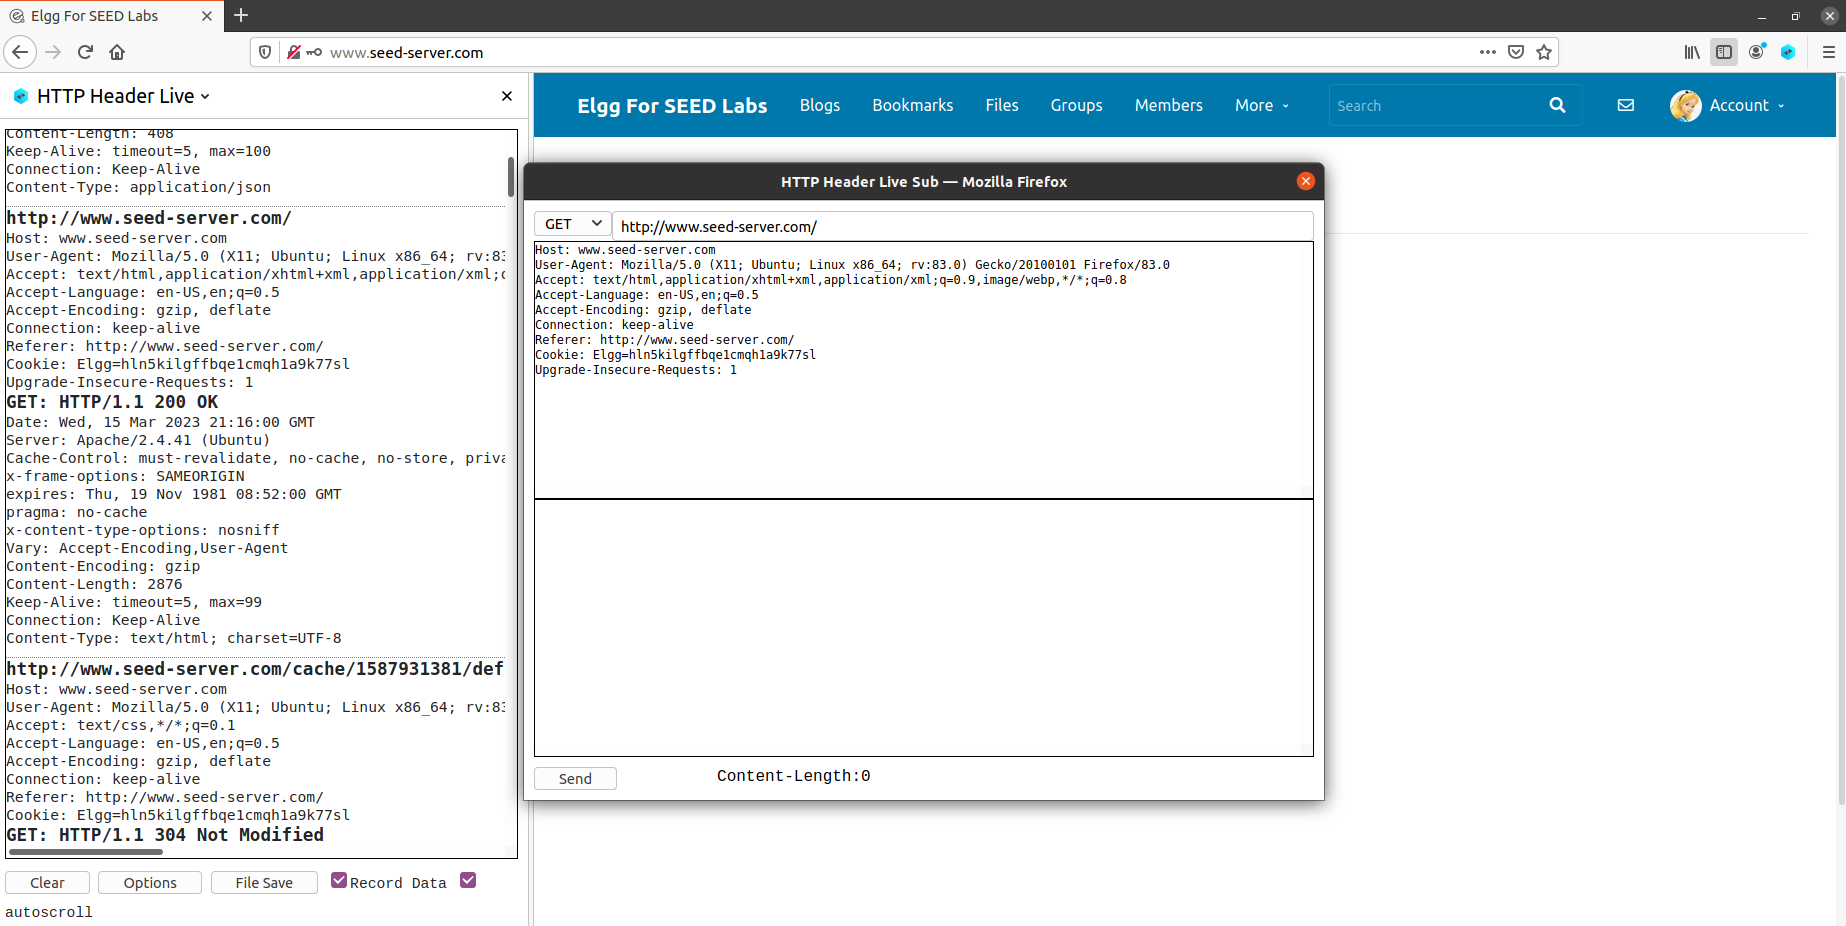
\includegraphics[width=\textwidth,height=\textheight,keepaspectratio]
    {figures/HTTP_GET.png}
    \caption{HTTP GET request in Elgg.}\label{fig:http_get}
\end{figure}

\begin{figure}
    \centering
    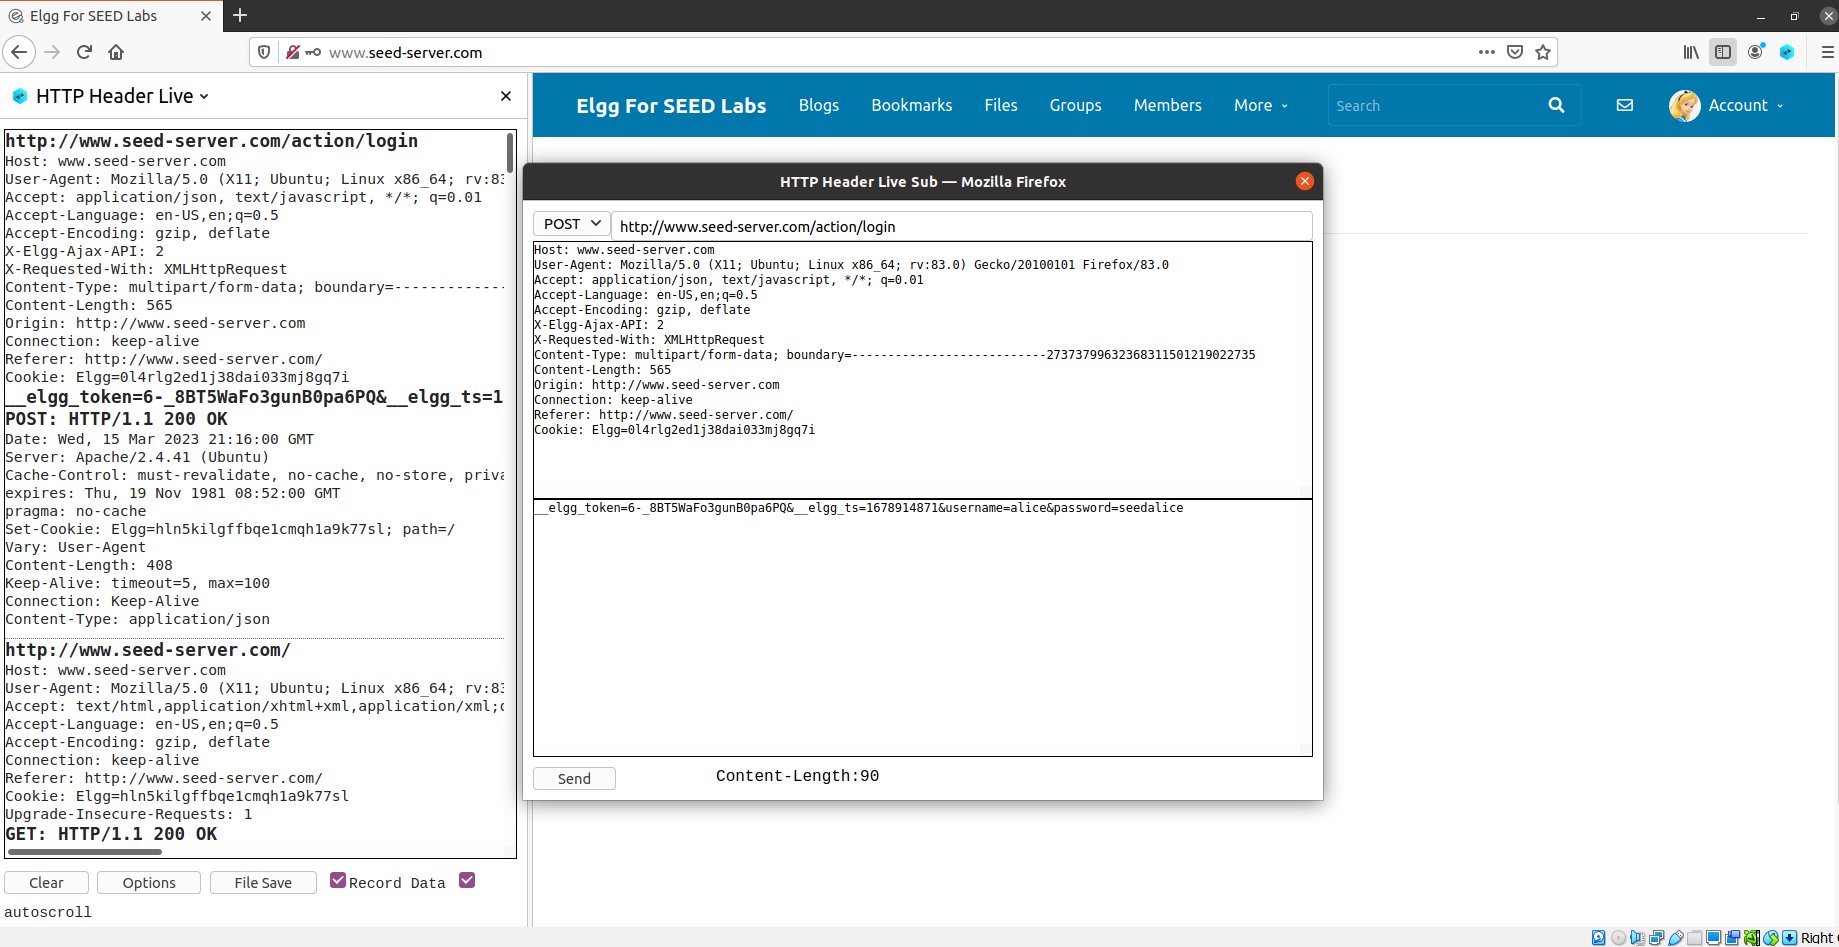
\includegraphics[width=\textwidth,height=\textheight,keepaspectratio]
    {figures/HTTP_POST.png}
    \caption{HTTP POST request in Elgg.}\label{fig:http_post}
\end{figure}

In the HTTP POST request, in this case we was trying to log in with a valid
authentication (username: \emph{alice}, password: \emph{seedalice}), it requires
a pair of parameters:{\fontfamily{qcr}\selectfont username} and
{\fontfamily{qcr}\selectfont password} (see \autoref{fig:http_post}).
On the other hand, a HTTP GET request does not require any parameters
(see \autoref{fig:http_get}).
% ...
% \section{Task 2 --- Generating a Certificate Request for Your Web Server}
%
\begin{lstlisting}[language=bash,caption=A command generating CSR for the server]
openssl req -newkey rsa:2048 -sha256 \
    -keyout server.key -out server.csr \
    -subj "/CN=www.student22.com/O=Student22 Inc./C=US" \
    -passout pass:dees \
    -addext "subjectAltName = DNS:www.student22.com,\
                            DNS:www.student22cuong.com,\
                            DNS:www.student22mahibul.com"
\end{lstlisting}

\begin{figure}
    \centering
    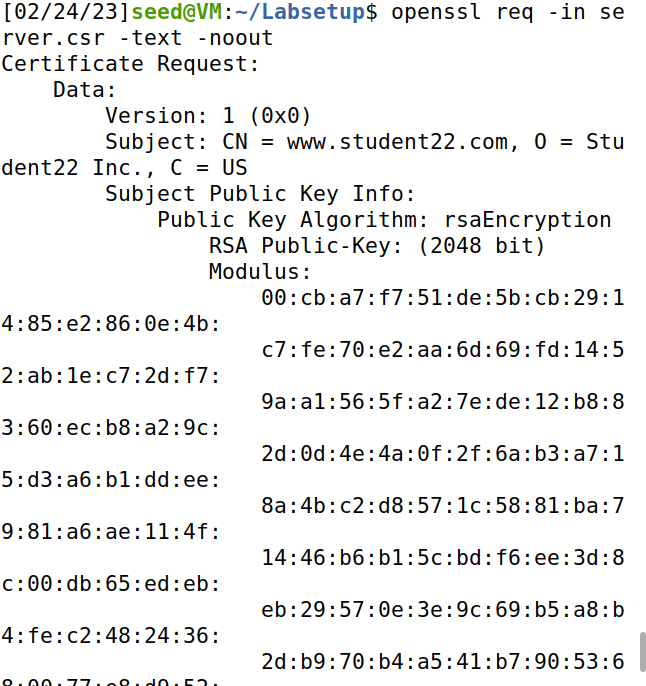
\includegraphics[height=\textheight,width=\textwidth,keepaspectratio]
    {figures/server_csr.png}
    \caption{Certificate Signing Request for the server
    {\fontfamily{qcr}\selectfont www.student22.com}.}
    \label{fig:server_csr}
\end{figure}

Two alternative names, {\fontfamily{qcr}\selectfont www.student22cuong.com} and
{\fontfamily{qcr}\selectfont www.student22mahibul.com}, are included
in the {\fontfamily{qcr}\selectfont openssl ca} command.
\autoref{fig:server_csr} shows partly the Certificate Signing Request
(CSR) for the server {\fontfamily{qcr}\selectfont www.student22.com}.
\section{Lab Tasks: Attacks}
\subsection{Task 1 --- Observing HTTP Request}
%
\begin{figure}
    \centering
    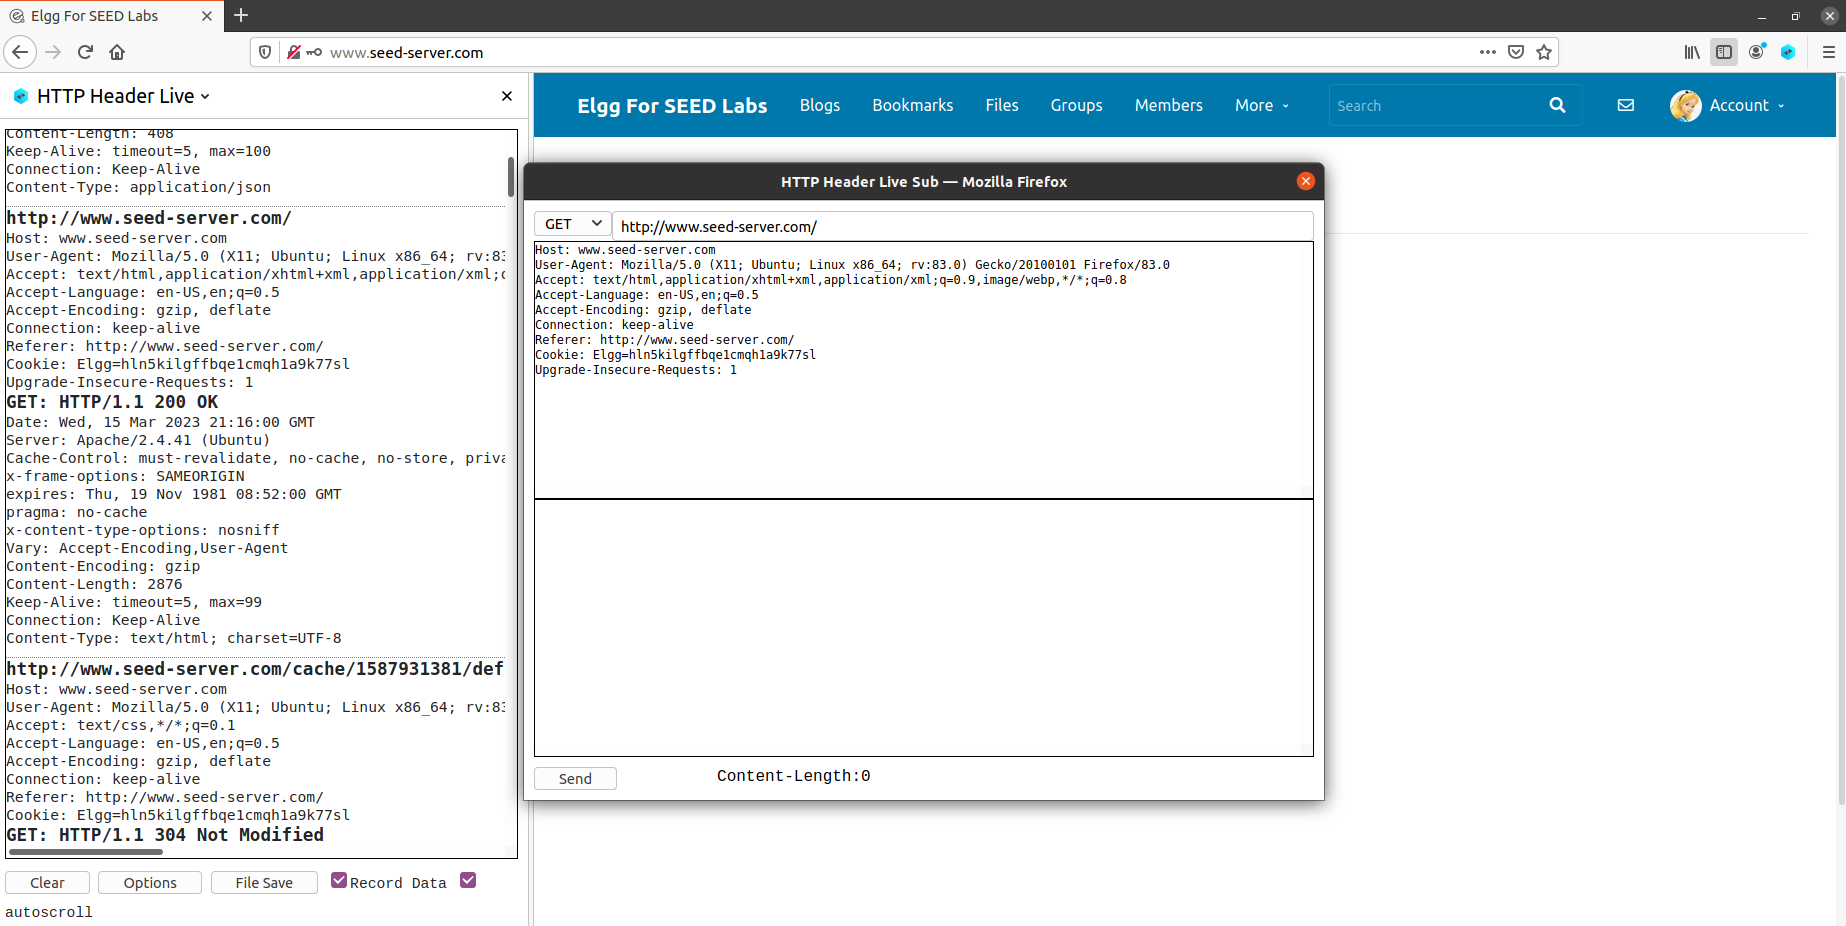
\includegraphics[width=\textwidth,height=\textheight,keepaspectratio]
    {figures/HTTP_GET.png}
    \caption{HTTP GET request in Elgg.}\label{fig:http_get}
\end{figure}

\begin{figure}
    \centering
    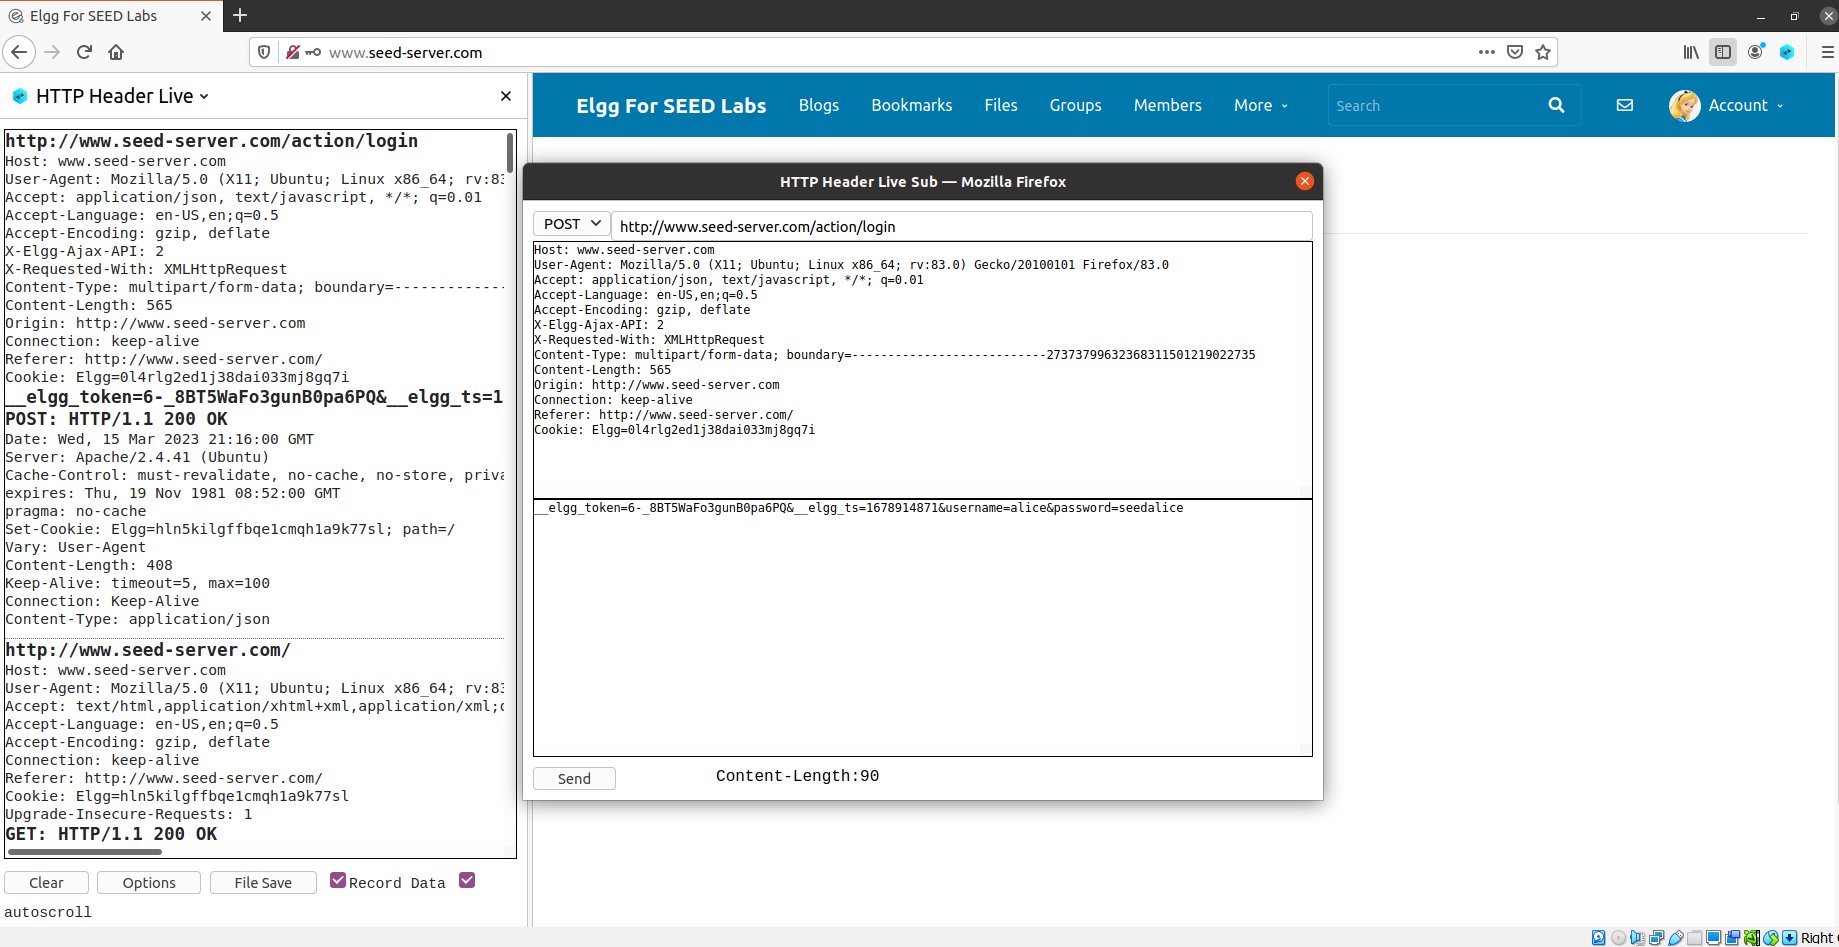
\includegraphics[width=\textwidth,height=\textheight,keepaspectratio]
    {figures/HTTP_POST.png}
    \caption{HTTP POST request in Elgg.}\label{fig:http_post}
\end{figure}

In the HTTP POST request, in this case we was trying to log in with a valid
authentication (username: \emph{alice}, password: \emph{seedalice}), it requires
a pair of parameters:{\fontfamily{qcr}\selectfont username} and
{\fontfamily{qcr}\selectfont password} (see \autoref{fig:http_post}).
On the other hand, a HTTP GET request does not require any parameters
(see \autoref{fig:http_get}).
\section{Task 2 --- Generating a Certificate Request for Your Web Server}
%
\begin{lstlisting}[language=bash,caption=A command generating CSR for the server]
openssl req -newkey rsa:2048 -sha256 \
    -keyout server.key -out server.csr \
    -subj "/CN=www.student22.com/O=Student22 Inc./C=US" \
    -passout pass:dees \
    -addext "subjectAltName = DNS:www.student22.com,\
                            DNS:www.student22cuong.com,\
                            DNS:www.student22mahibul.com"
\end{lstlisting}

\begin{figure}
    \centering
    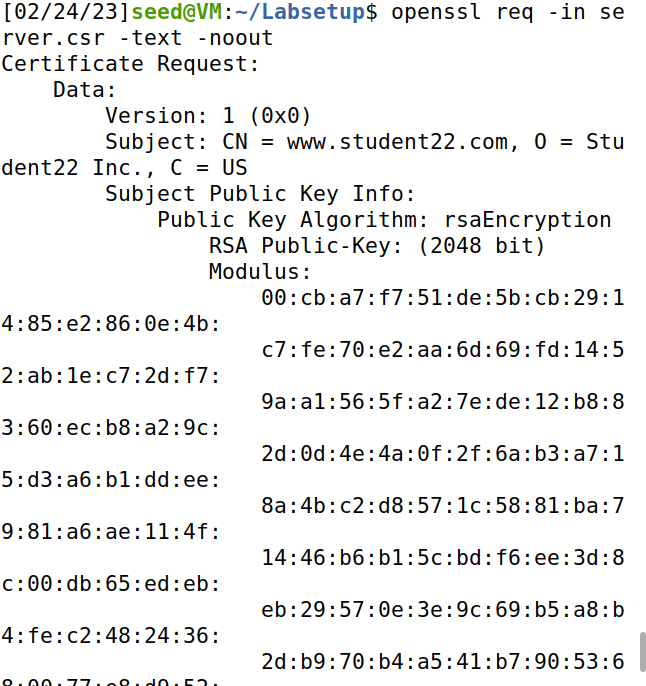
\includegraphics[height=\textheight,width=\textwidth,keepaspectratio]
    {figures/server_csr.png}
    \caption{Certificate Signing Request for the server
    {\fontfamily{qcr}\selectfont www.student22.com}.}
    \label{fig:server_csr}
\end{figure}

Two alternative names, {\fontfamily{qcr}\selectfont www.student22cuong.com} and
{\fontfamily{qcr}\selectfont www.student22mahibul.com}, are included
in the {\fontfamily{qcr}\selectfont openssl ca} command.
\autoref{fig:server_csr} shows partly the Certificate Signing Request
(CSR) for the server {\fontfamily{qcr}\selectfont www.student22.com}.

\printbibliography{}

\end{document}